 \def\us{\char`\_}


\subsection{WR link model}
\label{s:link_model}

Knowledge of the physical model of the links connecting the clocks is a
prerequisite for achieving the required synchronization accuracy. The model
of a WR optical link is depicted in Figure~\ref{fig:link_model}.
\begin{figure}[ht!]
  \centering
  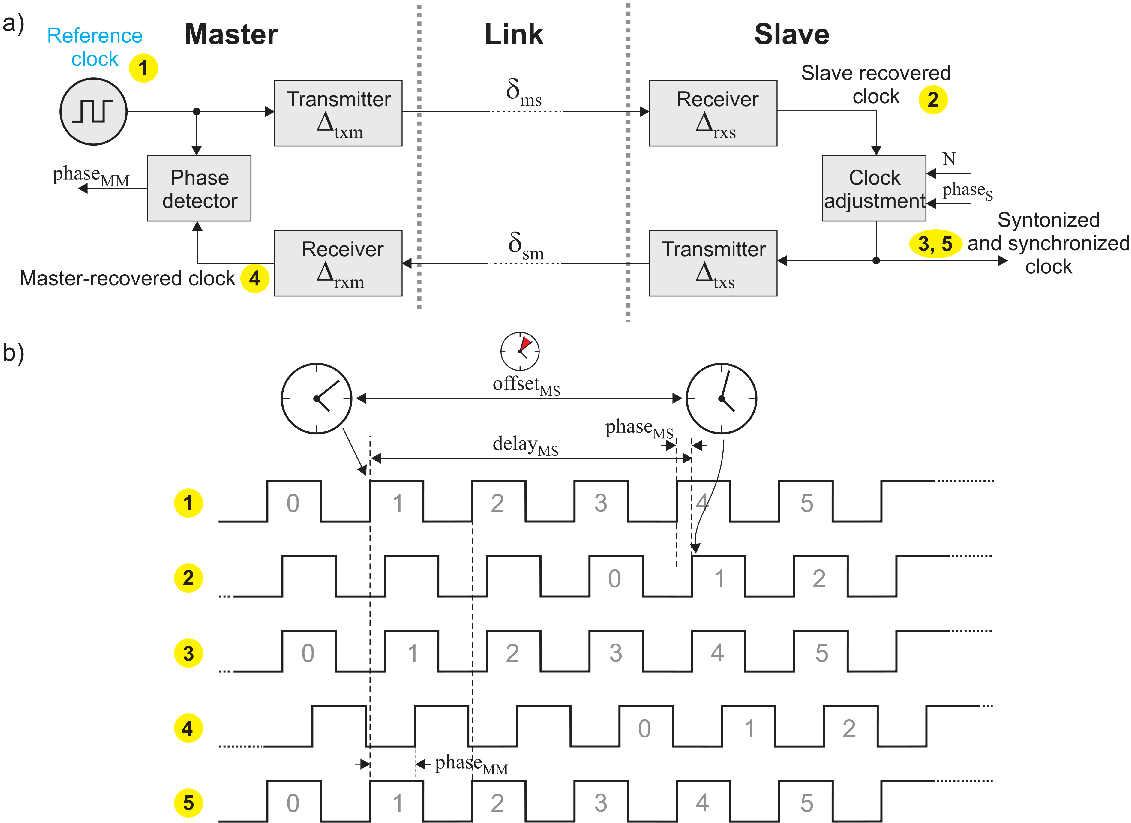
\includegraphics[width=15cm]{protocol/link_model.pdf}
  \caption{Model of a WR link (a) and relations between master and slave
  clocks (b)}
  \label{fig:link_model}
\end{figure}
[...]
% \textit{Delta} values shown in Figure~\ref{fig:link_model} express the delays
% introduced by various elements of the system. Big deltas ($\Delta_{txm},
% \Delta_{rxs},  \Delta_{txs},  \Delta_{rxm}$) indicate constant delays
% (e.g. the delays which never change when the link is active), while small
% deltas ($\delta_{ms}, \delta_{sm}$) express the delays which can vary during
% the operation of the link.

WR employs the clock loopback technique to measure the round-trip phase shift
$phase_{MM}$, which is a starting point for determining the precise two-way
delay $delay_{MM}$ and thus the clock offset $offset_{MS}$. The clock signal is
transferred between the master and the slave according to the following scheme:
\begin{enumerate}
\item The reference clock (1) is used to encode the master's transmitter
output and then extracted from the data stream at the slave's receiver. The
recovered clock (2) is a copy of clock (1) delayed by $delay_{MS}$, where
\begin{equation}
    \label{eq:delayms2}
    delay_{MS} = \Delta_{txm} + \delta_{ms} + \Delta_{rxs}
\end{equation}
expresses the master-to-slave latency introduced by the transceivers and
the link.
\item The recovered clock (2) is fed to a clock adjustment unit which shifts
its phase by a programmable value $phase_{S}$ to obtain the phase-compensated
clock (3) -- the final result of WR synchronization.
\item Clock (3) encodes the slave's outgoing data stream and is recovered
at the master side as signal (4).
\item The master measures the phase shift $phase_{MM}$ between its outgoing
(1) and incoming (4) clocks using a phase detector.
\end{enumerate}
The value of $phase_{MM}$ can be expressed as:
\begin{equation}
    \label{eq:phasemm}
    phase_{MM} = \{\Delta + \delta_{ms} + \delta_{sm} + phase_{S}\} \bmod
    T_{ref}
\end{equation}
where $\Delta = \Delta_{txm} + \Delta_{rxs} + \Delta_{txs} + \Delta_{rxm}$
and $T_{ref}$ is the period of Gigabit Ethernet 125 MHz reference clock (8 ns).

The goal of the presented model is to calculate the precise value of
master-to-slave offset $offset_{MS}$ by combining a coarse timestamp-based
round-trip delay \eqref{eq:meanPath} with precise phase measurement
$phase_{MM}.$ Once the offset is computed, the WR slave can phase-shift its
recovered clock (deriving $phase_{S}$ from $offset_{MS}$) to match the phase
of the master clock, completing the synchronization.
\begin{figure}[ht!]
  \centering
  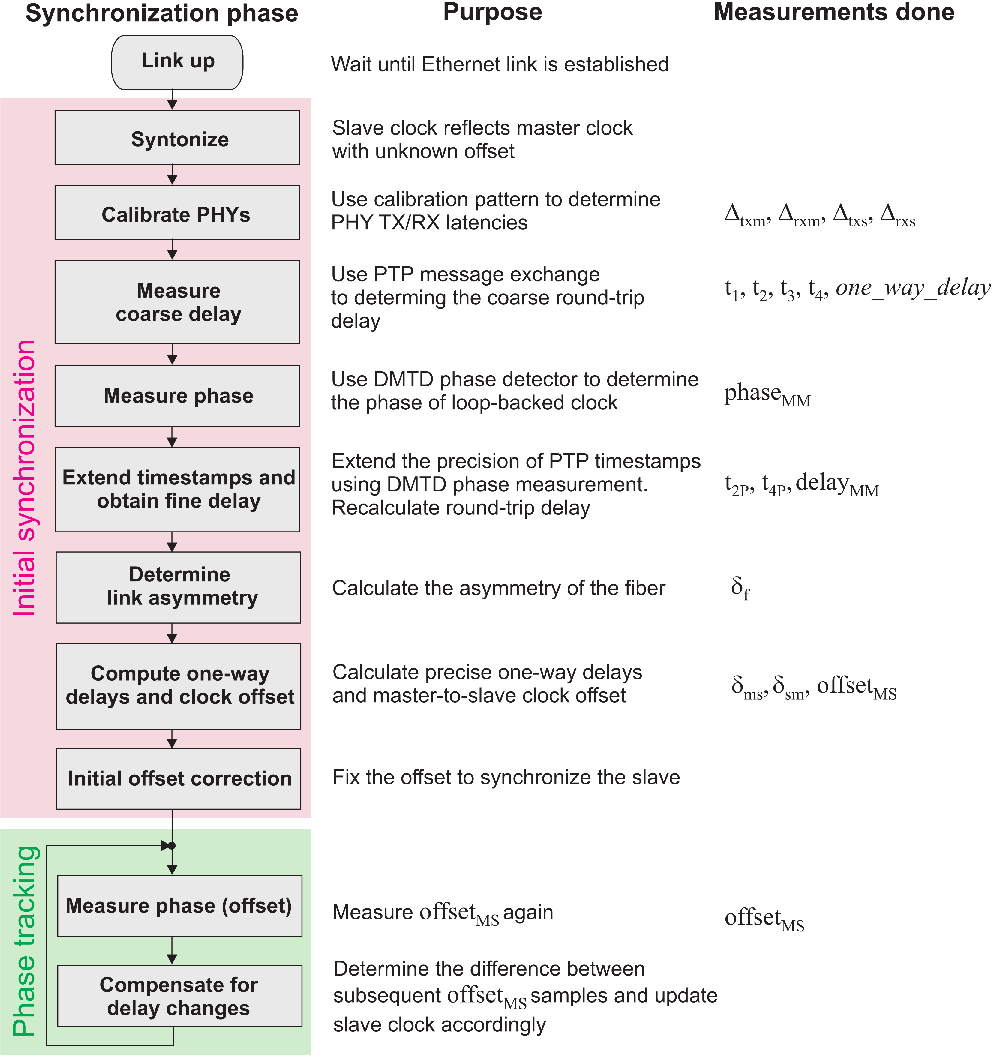
\includegraphics[width=15cm]{protocol/sync_flow.pdf}
  \caption{WR synchronization flow (DMTD is explained in Appendix~\ref{s:dmtd})}
  \label{fig:sync_flow}
\end{figure}
Determining the precise offset, however, is not a trivial task. Figure
\ref{fig:sync_flow} shows the steps needed to achieve and maintain
synchronization of a single WR link. The synchronization process can be
split into two parts: \begin{itemize}
\item \textbf{initial synchronization}, which determines the value of
$offset_{MS}$ and fixes the slave's phase shift to compensate the offset.
\item \textbf{phase tracking} which monitors the changes of $phase_{MM}$
over time and updates the phase shifter in the slave to follow these changes
and sustain synchronization.
\end{itemize}

\newpage

\subsection{Link detection and syntonization}
During the first two steps of the synchronization flow
\ref{fig:sync_flow}, a syntonized WR connection is established. Drawing
\ref{fig:link_detect_and_syntonization} shows the order of hardware operations
and message exchanges which result in a syntonized link.
\begin{figure}[ht!]
  \centering
  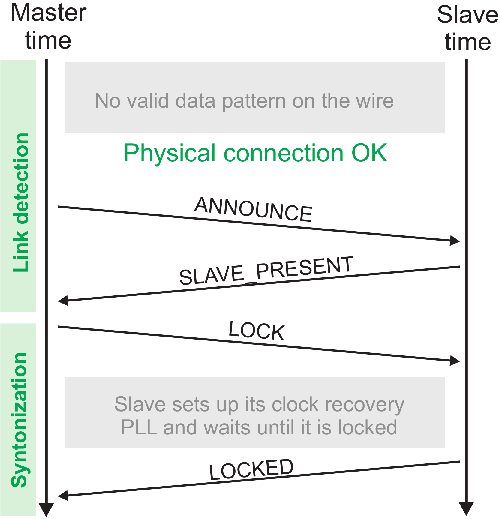
\includegraphics[width=7cm]{protocol/link_detect_and_syntonization.pdf}
  \caption{WR Link detection and syntonization}
  \label{fig:link_detect_and_syntonization}
\end{figure}
At the initial moment, the master and the slave are not connected to
each other. Their PHYs are transmitting an Ethernet idle pattern (see Table 3.1 \cite{tomekMSC}), 
but are not receiving any meaningful bitstreams. As soon
as the physical connection is present, the PHYs will start receiving valid
idle patterns and the Ethernet link will become active (see \cite{IEEE802.3}
section 36.2.5.2.6). Presence of a valid physical link will trigger the
following sequence:
\begin{enumerate}
\item The master starts broadcasting \textit{ANNOUNCE} messages to look for
a WR slave,
\item Eventually, the slave will respond with a \textit{SLAVE\_PRESENT}
message, indicating that it supports WR. If no response has been received
within a predefined time, the master assumes that the slave is not WR
compatible and aborts the synchronization process,
\item The master issues a \textit{LOCK} message, commanding the slave to
begin recovering the clock from its received data stream,
\item The slave sets up its PLL to use the RX clock as a reference and as
soon as the PLL is locked, responds with a \textit{LOCKED} message.
\end{enumerate}
Upon successful completion of the above process, both nodes are syntonized
and the delay measurements can begin.

\subsection{Coarse delay measurement}
\label{s:coarse_delay}
The coarse delay measurement produces a set of timestamps $t_{1} ... t_{4}$
which are obtained using the PTP End-to-End, two-way clock method as shown
in fig. \ref{fig:wrPTPmsgs}. The timestamps are generated in the hardware
with a circuit depicted in fig. \ref{fig:coarse_measurement}, guaranteeing
single-cycle timestamping accuracy, which is necessary for reliably merging the
coarse delay with the $phase_{MM}$ phase shift during fine delay calculation.
\begin{figure}[ht!]
  \centering
  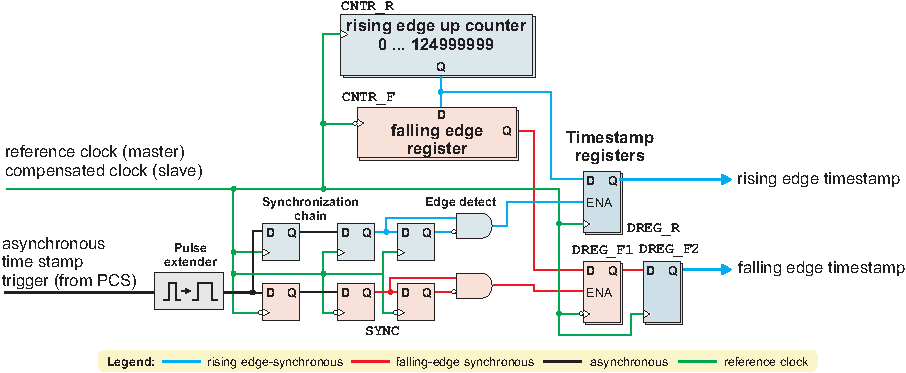
\includegraphics[width=17cm]{protocol/coarse_measurement.pdf}
  \caption{Structure of a WR timestamping unit (TSU)}
  \label{fig:coarse_measurement}
\end{figure}
Timestamps in WR are taken when the PCS detects a Start-of-Frame Delimiter
(SFD) character in the incoming (RX timestamps) or outgoing (TX timestamps)
data stream (see section 3.2.2 \cite{tomekMSC}).

Let's first focus on the blocks marked blue in
Figure~\ref{fig:coarse_measurement}. Each time an SFD character is detected,
the PCS produces a timestamp trigger pulse which causes the timestaming unit
to take a snapshot of the free running counter CNTR\_R with the D-type
register DREG\_R. The counter is counting from 0 to 124999999 which (given
the reference clock frequency of 125 MHz) gives a period of one full second.

The counter CNTR\_R works synchronously to the reference clock (master side,
signal 1 in Figure~\ref{fig:link_model}) or the compensated clock (slave side,
signal 5). Since RX trigger pulses come from different clock domains (2 or
4), they need to be synchronized to the reference clock with a chain of
D flip-flops (SYNC). Single-cycle long trigger pulses are widened by the
pulse extender before going to the synchronizer chain to ensure that no
pulses are missed due to the metastability of synchronizer flip-flops. The
counter value is latched in register DREG\_R on the rising edge of the
synchronizer output. TX timestamp triggers, which are generated within the
reference clock domain (clocks 1 or 5) also pass through a synchronizer
chain to obtain identical trigger reaction latency.

Unfortunately, due to the jitter of clock signals, crossing clock domains
can make the gathered timestamps useless by causing a random $\pm 1$ LSB
error when the RX clock and the reference clocks are almost in phase. The
problem is illustrated in Figure~\ref{fig:ts_jitter}.  Dashed lines show
the transitions of ideal (jitter-free) clocks. If the jitter is neglected,
the reference clock transition should be slightly ahead of the RX clock
transition and the gathered timestamp should be equal to 2. However, if the
clocks are jittery, the transitions may sometimes occur in reverse order,
producing an erroneous timestamp of value 1.
\begin{figure}[ht!]
  \centering
  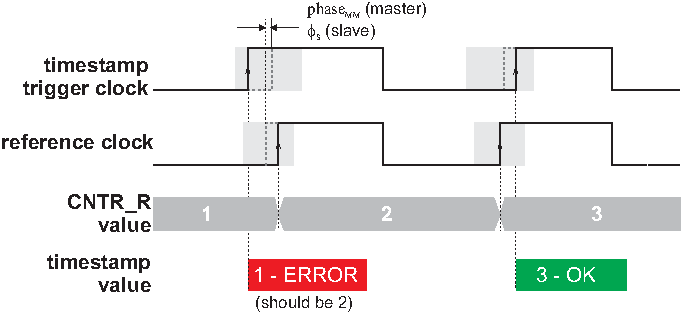
\includegraphics[width=10cm]{protocol/ts_jitter.pdf}
  \caption{Timestamping errors caused by clock jitter}
  \label{fig:ts_jitter}
\end{figure}
One possible way of addressing this issue is to take RX timestamps on both
reference clock edges. The falling edge part of the TSU is marked pink in
\ref{fig:coarse_measurement}. It does not have an independent counter --
instead, the current value of the rising edge counter is latched in register
CNTR\_F on the falling edge of the reference clock, making the CNTR\us
F a copy of CNTR\_R delayed by a half of the clock period. This method
ensures that at least one of the timestamps is valid at any moment 
(see Figure~\ref{fig:ts_dualedge}). The correct timestamp is chosen depending on the
current phase shift between clocks (see section \ref{s:fine_delay}).
\begin{figure}[ht!]
  \centering
  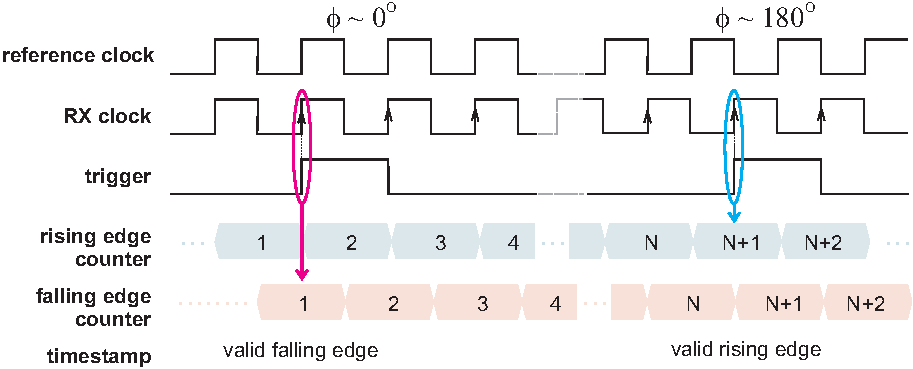
\includegraphics[width=12cm]{protocol/ts_dualedge.pdf}
  \caption{Dual-edge timestamping in WR}
  \label{fig:ts_dualedge}
\end{figure}
In order to simplify the hardware design, the presented TSU can only measure
the sub-second part of PTP timestamps. The UTC part is appended in the
software using the algorithm shown in listing \ref{lst:utc_gen}.
\begin{lstlisting}[caption=Producing UTC timestamps,label=lst:utc_gen]
  timestamp tstamp = get_hardware_timestamp();
  time t = get_utc_time();
// check if there was a transition of the UTC counter between the
// generation of the timestamp and its readout by the software
  if(t.milliseconds < tstamp.rising_edge)
   tstamp.seconds = t.seconds - 1;
  else
   tstamp.seconds = t.seconds;
\end{lstlisting}


\subsection{Digital DMTD phase detector}
\label{s:dmtd}
The fine delay measurements in WR are based on a Dual Mixer Time Difference
(DMTD) phase detector. Therefore, in this section a short introduction to
DMTD technology will be presented.
\begin{figure}[ht!]
  \centering
  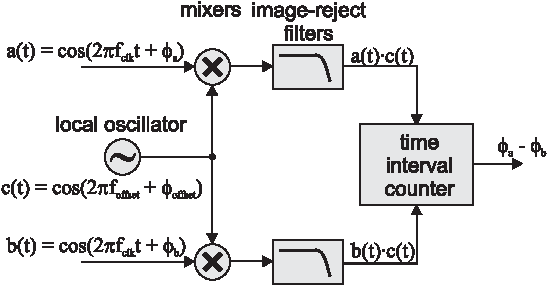
\includegraphics[width=11cm]{misc/analog_dmtd.pdf}
  \caption{Structure of an analog DMTD phase detector}
  \label{fig:analog_dmtd}
\end{figure}
Figure \ref{fig:analog_dmtd} shows an analog DMTD system \cite{allan90}. Let's
assume that its input clocks $a(t)$ and $b(t)$ have identical amplitudes and
frequencies equal to $f_{clk}$. The phases of both clocks are respectively
$\phi_{a}$ and $\phi_{b}$. The clocks are multiplied by the mixers with
the signal $c(t)$ of frequency $f_{offset}$ and phase $\phi_{offset}$. The
multiplication result can be expressed as:

\begin{eqnarray}
    a(t) \cdot c(t) & = & cos(2\pi t f_{clk} + \phi_{a}) \cdot cos (2\pi t
    f_{offset} + \phi_{offset}) \nonumber \\
\label{eq:mixing1}& = & \frac{1}{2} cos(2\pi t (f_{clk} + f_{offset}) +
\phi_a + \phi_{offset}) \\
\label{eq:mixing2}& + & \frac{1}{2} cos (2 \pi t (f_{clk} - f_{offset}) +
\phi_a - \phi_{offset})
\end{eqnarray}

Term \ref{eq:mixing1} has higher frequency than the multiplied signals and
it's removed by the low-pass filter, leaving only the low-frequency term
\ref{eq:mixing2}. The downconversion process changes the frequency of the
signals, but does not change their phase difference. Therefore, if the offset
frequency $f_{offset}$ is close to the input signal frequency $f_{clk}$,
the phase shift can be measured by counting the time between the rising
edges of the downconverted clocks. For example, a reference clock of 125
MHz and an offset clock of 124.99 MHz will produce an output signal of 10
kHz. At such frequencies, the phase shift can be very accurately measured
using a simple counter.

Analog DMTDs provide excellent resolution and linearity, at the cost of several
external discrete components (mixers and filters), which can be troublesome,
especially in multi-port applications such as the WR switch. Fortunately, the
analog mixing operation can be transformed into a digital sampling operation,
resulting in a digital DMTD detector, shown on fig. \ref{fig:digital_dmtd}.
\begin{figure}[ht!]
  \centering
  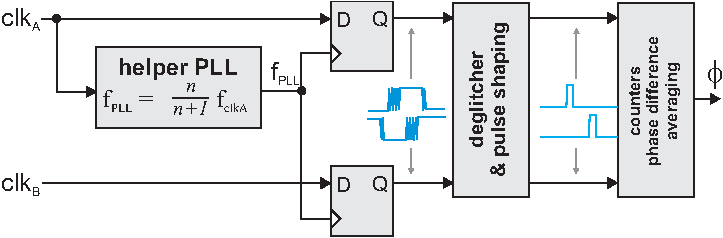
\includegraphics[width=12cm]{misc/dmtd.pdf}
  \caption{Structure of a digital DMTD phase detector}
  \label{fig:digital_dmtd}
\end{figure}
In a Digital DMTD (DDMTD) \cite{icalepcs09}, the input signals are square
waves, the mixers are replaced with simple D-type flip-flops and the offset
clock is generated with a PLL from one of the input clocks. The sampling
operation performed by the flip-flops can be mathematically proved to be
equivalent to analog mixing (\ref{eq:mixing2}), but the principle of a DDMTD
can be explained in a more intuitive way.
\begin{figure}[ht!]
  \centering
  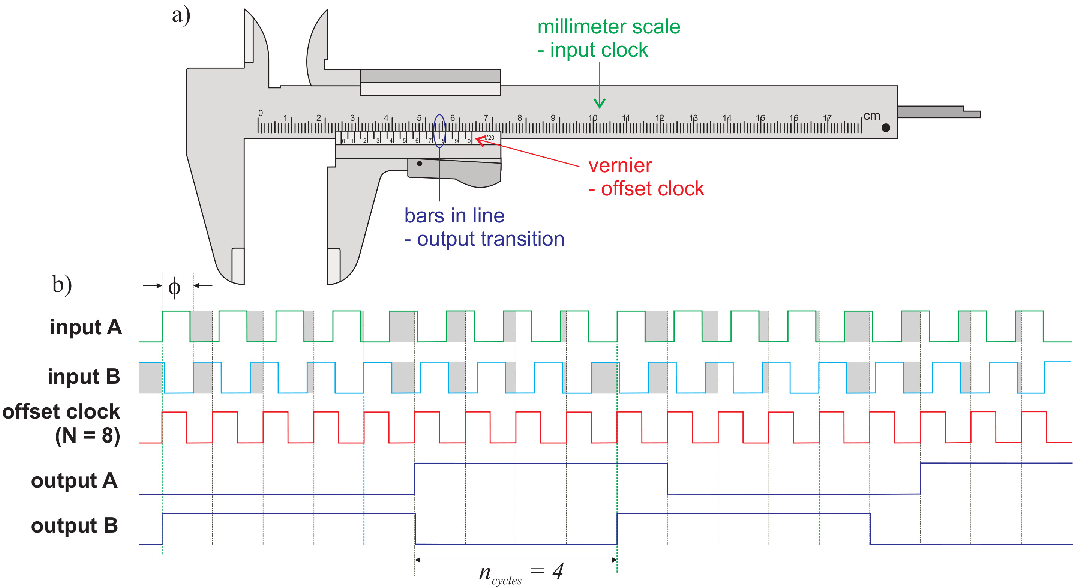
\includegraphics[width=15cm]{misc/dmtd_vernier.pdf}
  \caption{A vernier (a) and signals generated by DDMTD (b)}
  \label{fig:dmtd_vernier}
\end{figure}
Figure \ref{fig:dmtd_vernier}a shows a vernier caliper. It has two scales -
the big millimeter scale and a small vernier scale, with the units slightly
smaller than the main scale. For a typical caliper, the vernier scale is split
into 10 intervals with 4.9 mm spacing. If the length of the measured object
has a fractional part, one of bars on the vernier scale will be in line with
one of bars from the main scale. Translating to the language of electronics,
the main scale is the input clock where each interval represents one cycle,
the vernier scale is the offset clock and the transitions in the DDMTD output
signals occur when bars on both scales are aligned. An example of signals
produced by a DDMTD with $N = 8$ is shown in fig. \ref{fig:dmtd_vernier}b. The
output phase shift is proportional to the input phase shift $\phi$ by a
factor of $(N+1)$. A general relation between the phase shift and the cycle
interval between the DMTD outputs can be expressed as:

\begin{equation}
\label{eq:dmtd1}
\phi \mbox{[ns]} = \frac{n_{cycles}}{N+1} \cdot \frac{1}{f_{in}}
\end{equation}


Digital DMTDs have all the advantages of their analog counterparts while
requiring only one external component (the oscillator producing the offset
clock) which is shared among all measurement channels.	This opens the way
for low-cost FPGA implementations. If a picosecond-level accuracy is not
required, even a PLL integrated inside an FPGA can be used, eliminating all
external components.
\begin{figure}[ht!]
  \centering
  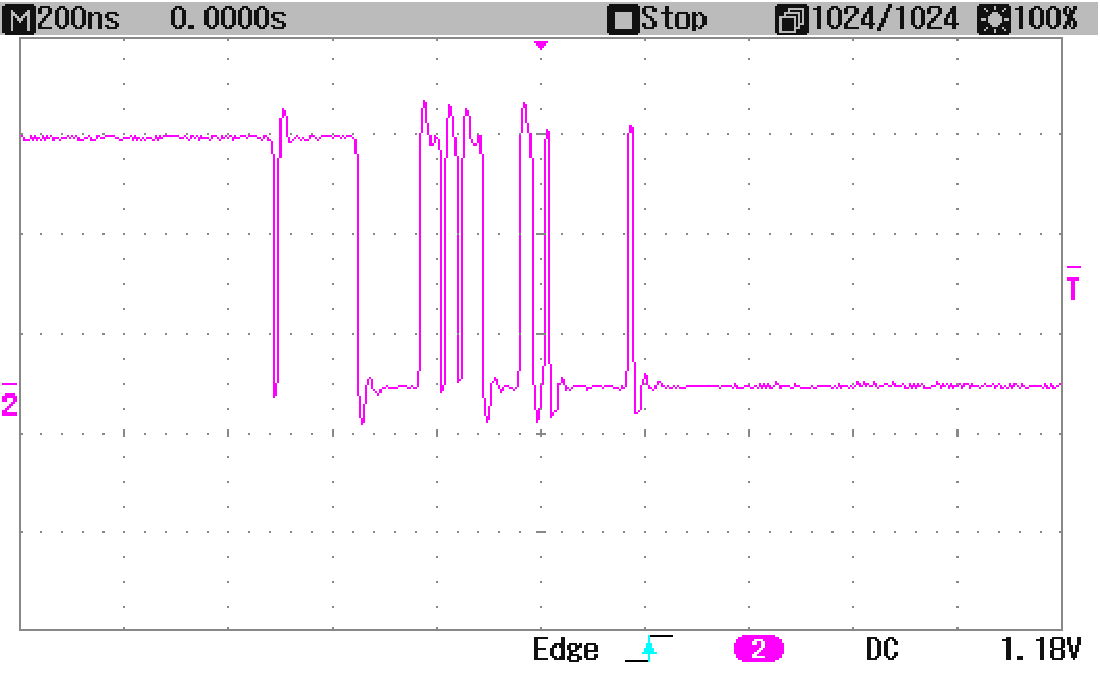
\includegraphics[width=8cm]{misc/dmtd_glitches.pdf}
  \caption{Glitches in the DMTD output caused by clock jitter}
  \label{fig:dmtd_glitches}
\end{figure}
In practical DDMTD implementations, the output signals need to be additionally
conditioned as the input clock jitter can introduce glitches, as shown
on fig. \ref{fig:dmtd_glitches}. More details about the deglitching and
postprocessing algorithm can be found in section 4.3.5 of \cite{tomekMSC}.

\subsection{Fine delay measurement}
\label{s:fine_delay}
Having the knowledge of PTP timestamps and round-trip phase shift $phase_{MM}$,
we can calculate the precise round-trip delay $delay_{MM}$. The calculation
is performed in two steps:
\begin{itemize}
\item The accuracy of PTP timestamps $t_{2}$ and $t_{4}$ is enhanced beyond a
single clock cycle using the knowledge of the round-trip phase $phase_{MM}$
and the slave PLL setpoint $phase_{S}$. As a result, precise timestamps
$t_{2p}$ and $t_{4p}$ are obtained.
\item The fine round-trip delay is calculated using the standard PTP formula:
\begin{equation}
\label{eq:ptp_precise}
delay_{MM} = (t_{4p} - t_{1}) - (t_{3} - t_{2p})
\end{equation}
\end{itemize}

Only the reception timestamps need to be enhanced, as they are generated
within clock domains asynchronous to the reference (or compensated) clock
(see table \ref{tab:ts_domains}). Transmission timestamps are always integer
because packets are transmitted and timestamped using the same clock.

The flow graph of the algorithm used to merge PTP timestamps with
phase measurements is shown on Figure~\ref{fig:merging_timestamps}. 
Figure~\ref{fig:merging_example} depicts sample measurements of inputs and results
of the enhancement algorithm for $t_{4p}$ timestamps, where the varying link
delay was simulated using the slave's phase shifter.

\begin{table}[htb]
  \caption{Timestamping clock domains}
  \centering
  \begin{tabular}{|c|c|c|c|c|} \hline
    Timestamp & Origin & Trigger clock & Timestamping clock & Correction \\
    \hline \hline
    $t_{1}$ & Master TX & reference (1) & reference (1) & 0 \\ \hline
    $t_{2p}$ & Slave RX & slave recovered (2) & compensated (3) & $-phase_{S}$
    \\ \hline
    $t_{3}$ & Slave TX & compensated (3) & compensated (3) & 0 \\ \hline
    $t_{4p}$ & Master RX & master recovered (4) & reference (1) & $+phase_{S}$
    \\ \hline
  \end{tabular}
  \label{tab:ts_domains}
\end{table}
\begin{figure}[ht!]
  \centering
  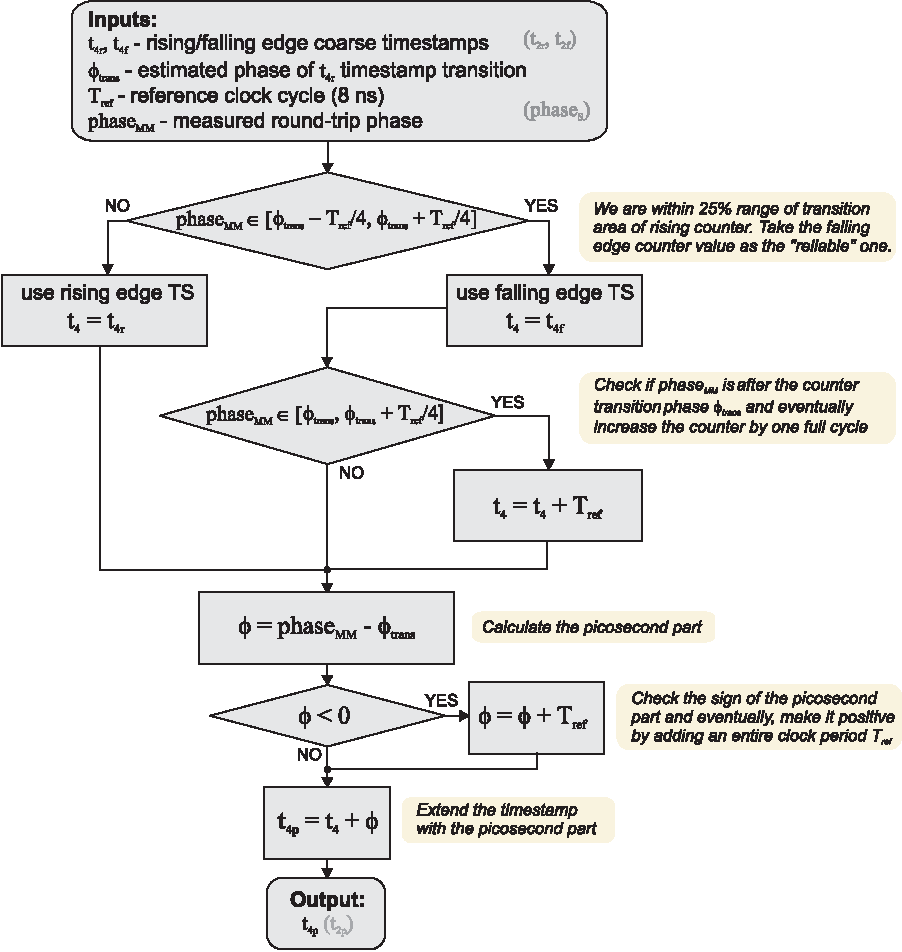
\includegraphics[width=13cm]{protocol/merging_timestamps.pdf}
  \caption{Algorithm for enhancing coarse timestamps with DMTD phase.}
  \label{fig:merging_timestamps}
\end{figure}
The first step of the algorithm addresses the problem of glitches in
RX timestamps, by choosing either the rising or falling edge timestamp
depending on the phase between the RX clock and the reference clock. The
key parameter of this step, $\phi_{trans}$ provides an approximate
value of $phase_{MM}$ at which a transition should occur in the value of
$t_{4r}$. In Figure~\ref{fig:merging_example}, it is equal to 6.6 ns - it's
the approximate intersection point of $phase_{MM}$ (blue, sawtooth-like
trace) and the transition of the rising edge timestamp (red trace). The
value of $\phi_{trans}$ is a device-specific constant. It can be determined
once during the factory calibration of a WR device or measured upon every
startup by sweeping a full clock period using the built-in phase shifter
and searching for a transition in the RX timestamp value.

If the actual value of $phase_{MM}$ lies within a $\pm 25\%  T_{ref}$
range from the transition point $\phi_{trans}$ (green zone in
\ref{fig:merging_example}), the algorithm will use the $t_{4f}$ timestamp,
otherwise the $t_{4r}$ timestamp will be taken (red zone). Note that because
$phase_{MM}$ is bounded to $\left[0, T_{ref}\right)$, the range checks must
be aware of the jump in the phase between $T_{ref}$ and $0$.

The second step checks if the $phase_{MM}$ value is ahead of the transition
point $\phi_{trans}$, and eventually increases the chosen timestamp by a full
cycle ($T_{ref}$). That ensures the transition in $t_{4}$ will always occur
when $phase_{MM} = \phi_{trans}$, eliminating the risk of transition glitches.

The last part of the algorithm simply adds the picosecond part (which is
the DMTD phase corrected with the transition offset $\phi_{trans}$) to
the coarse deglitched timestamp $t_{4}$. If the resulting picosecond part
($\phi$) is negative, an additional full cycle is added to the result. The
final output of the merging algorithm is shown in \ref{fig:merging_example}
as the thick navy trace.
 \begin{figure}[ht!]
  \centering
  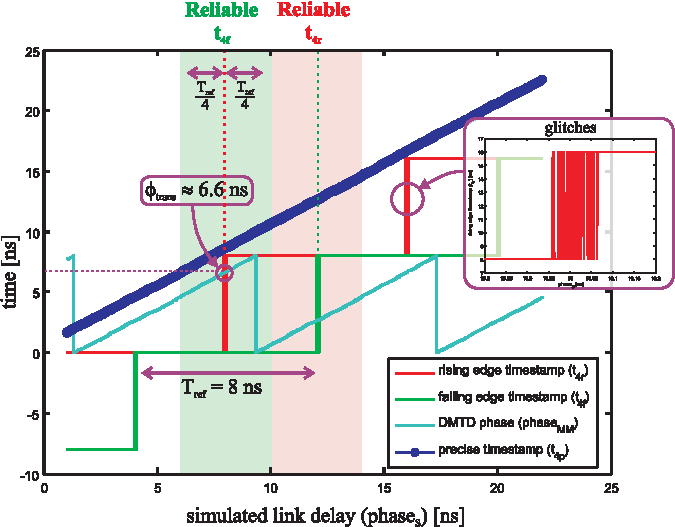
\includegraphics[width=12cm]{protocol/merging_example.pdf}
  \caption{Example of $t_{4p}$ timestamp enhancing.}
  \label{fig:merging_example}
\end{figure}
The enhancement operation for the $t_{2}$ timestamp is done in a very
similar way by replacing $t_{4}$ with $t_{2}$ and $phase_{MM}$ with
$phase_{S}$. Note that changing the slave's phase shift $phase_{S}$ will
result in a change of the values of both $t_{2p}$ and $t_{4p}$ (see table
\ref{tab:ts_domains}). Increasing $phase_{S}$ by a certain $\delta$ will
cause $t_{4p}$ to also increase by $\delta$ (assuming that the link delay
stays constant). Simultaneously, the value of $t_{2p}$ will be decreased by
the same amount, as for the slave's RX timestamps, the timestamping clock is
$phase_{S}$ ahead of the trigger clock (so if the phase shift is increased,
the timestamp value goes down). Therefore, the calculated fine delay is not
affected by the changes of $phase_{S}$:

\begin{equation}
\label{eq:ptp_precise2}
delay_{MM} = (t_{4p} - t_{1}) - (t_{3} - t_{2p}) = t_{4p} \cancel{+ phase_{S}}
- t_{1} - t_{3} + t_{2p} \cancel{-phase_{S}}
\end{equation}


\subsection{Link asymmetry estimation}
\label{s:asymmetry}
In order to compute an accurate master-slave offset, one must determine the
asymmetry of the link delay. This asymmetry cannot be measured directly (as
a difference between the overall M-S and S-M delays), as it would require
the nodes to be synchronized prior to the measurement. Therefore it is
only possible to estimate the asymmetry from round-trip delay $delay_{MM}$,
using the knowledge of the properties of the components constituting the link.

In the WR optical link model, the following sources of asymmetry were taken
into consideration:
\begin {itemize}
\item Propagation delays of electronic components and PCB traces (circuit
asymmetry),
\item Asymmetry of optical transceivers (SFPs),
\item Difference between TX and RX wavelengths in the fiber,
\item Internal structure and clocking of the PHY (SerDes) chips.
\end{itemize}
\begin{figure}[ht!]
  \centering
  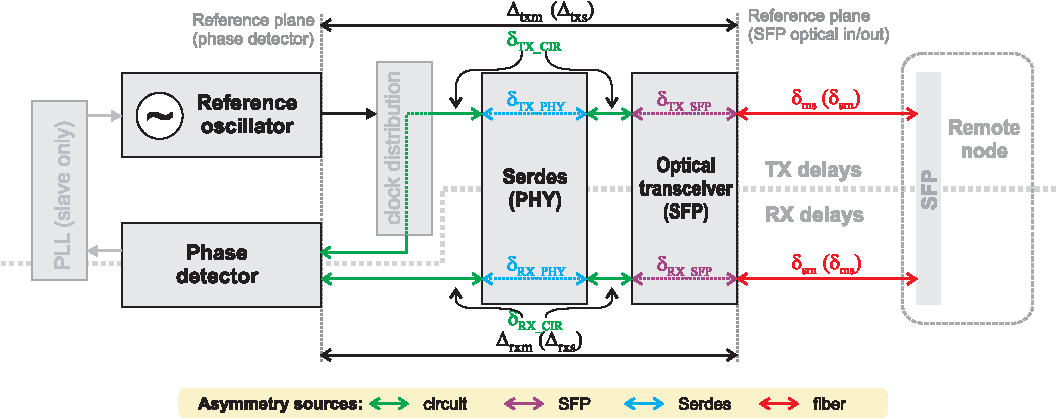
\includegraphics[width=\textwidth]{protocol/asymmetries.pdf}
  \caption{Delay asymmetries in WR optical link.}
  \label{fig:asymmetries}
\end{figure}
Figure \ref{fig:asymmetries} shows the reference asymmetry model used in WR
devices. The device's asymmetric delays (as shown in Figure~\ref{fig:link_model})
are expressed as sums of circuit, SFP and PHY delays between the phase detector
inputs (the PD measuring $delta_{MM}$ on the master side and the PD in the
phase shifting PLL on the slave side) and the SFP optical input/output. The
fiber asymmetry is compensated separately in the slave's PTP servo.
\begin{eqnarray}
\Delta_{tx(m/s)} = \delta_{TX\us PHY(M/S)} + \delta_{TX\us CIR(M/S)} +
\delta_{TX\us SFP(M/S)}
\\
\Delta_{rx(m/s)} = \delta_{RX\us PHY(M/S)} + \delta_{RX\us CIR(M/S)} +
\delta_{RX\us SFP(M/S)} \nonumber
\label{eq:asym_delay}
\end{eqnarray}\\

\subsubsection{Circuit and SFP asymmetry}
Circuit asymmetry stems from differing PCB trace lengths, propagation delays
of the electronic components of the clock distribution system and FPGA logic
cell placement and routing delays. SFP asymmetry is a result of different
reception and transmit delays between the electrical and optical ports of
the SFP transceiver.

These asymmetries can vary with changes of the device's operating conditions
(i.e. temperature, supply voltage). Depending on the synchronization accuracy
requirements, they can be:
\begin{itemize}
\item Treated as time-invariant and measured once during factory setup.
\item Actively compensated, following the changes in temperature and/or supply
voltage read from built-in sensors (requires a model of delay vs. temperature
and voltage),
\item Eliminated by building a system where both master and slave have
identical (or zero) asymmetry and operate in similar conditions.
\end{itemize}

The last method is particularly useful for compensating the delays inside
the FPGA on the way between the PHY (oscillator) and the phase detector,
as they cannot be externally measured during the factory calibration
process. They are also significantly affected by temperature and voltage
changes. Therefore, the only practical way of dealing with the FPGA part
of the circuit asymmetry is to equalize the delays on all phase detector
inputs. This can be done by constraining the routing delays or manually
placing and routing the phase detector block. This approach also allows for
reducing the impact of the temperature-voltage changes on the asymmetry to
a negligible value, as two equal paths placed next to each other would have
very similar temperature/voltage delay coefficients.

SFP asymmetries can be compensated in a similar manner by choosing pairs
of SFP transceivers whose TX and RX delays differ by similar values
(i.e. $\delta_{TX\us SFPM} - \delta_{RX\us SFPM} = \delta_{TX\us SFPS} -
\delta_{RX\us SFPS}$). This can be done in a laboratory system where all
other asymmetric delays are already compensated by selecting SFPs that
together give minimum clock offset.

\subsubsection{WDM fiber asymmetry}
\label{s:wdm_asymmetry}
As mentioned in section 3.2 of \cite{tomekMSC}, WR uses different wavelengths
for transmitting and receiving the data (for example 1550/1310 nm). Due
to chromatic dispersion of the fiber, the refractive indexes for these
wavelengths are slightly different, causing different propagation speeds
(and thus, different delays) between the master and the slave.

The refractive index at a given wavelength can be derived using Sellmeier's
equation  \cite{saleh07} (\ref{eq:sellmeier}):

\begin{equation}
\label{eq:sellmeier}
n^2(\lambda) = 1 + \frac{B_{1} \lambda^2}{\lambda^2 - C_{1}} + \frac{B_{2}
\lambda^2}{\lambda^2 - C_{2}} + \frac{B_{3} \lambda^2}{\lambda^2 - C_{3}}
\end{equation}

where $B_{i}$ and $C_{i}$ are material-specific coefficients.

For a standard G.652 telecom fiber, the refractive indexes are respectively:
$n_{1550} = 1.467$ and $n_{1310} = 1.466$. In order to simplify the asymmetry
calculations in the hardware, the WR specification defines
a custom fiber asymmetry coefficient \eqref{eq:fiber_alpha1} expressing the
ratio between the M-S and S-M fiber propagation delays:

\begin{equation}
\label{eq:fiber_alpha1}
\alpha = \frac{\delta_{ms}}{\delta_{sm}} - 1 = \frac{n_{1550}}{n_{1310}} - 1
\end{equation}
Unfortunately, refractive indexes may vary slightly between different fiber
manufacturers, making the direct calculation of $\alpha$ unreliable. WR
can solve this problem by characterizing the fiber asymmetry using
laboratory measurements of $delay_{MM}$ (done by PTP) and clock offset
$offset_{MS}$ (done using an oscilloscope). The measurements are performed
when all the other asymmetries are already compensated. The value of
$\alpha$ \ref{eq:fiber_alpha3} is calculated by solving equation system
\ref{eq:fiber_alpha2}:
\begin{equation}
\label{eq:fiber_alpha2}
\begin{cases}
delay_{MM} = \delta_{ms} + \delta_{sm} + \Delta \\
offset_{MS} = \frac{\delta_{ms} - \delta_{sm}}{2}
\end{cases}
\end{equation}
where $\Delta$ accounts for all fixed delays in the path (i.e. $\Delta_{txm}
+ \Delta_{rxs} + \Delta_{txs} + \Delta_{rxm}$). Substitution of $\delta_{ms}$
and $\delta_{sm}$ with the results of \ref{eq:fiber_alpha2} gives the final
value of $\alpha$:
\begin{equation}
\label{eq:fiber_alpha3}
\alpha = \frac{delay_{MM}  - \Delta + 2\cdot offset_{MS}}{delay_{MM} -
\Delta - 2\cdot offset_{MS}}
\end{equation}

\subsubsection{Transceiver asymmetry}
\label{s:xcvr_asymmetry}
\label{sec:calibForGigbitE}
\textit{[This chapter has been modified to add clarity]}


Transceiver asymmetry is a result of the internal structure of the SerDes's
circuitry. Most of the SerDes chips nowadays are optimized for low power
consumption and fast locking to the incoming data stream. Unfortunately,
because of these optimizations, PHYs may not keep constant transmit/receive
latencies. The problem is illustrated in Figure~\ref{fig:phy_asymmetry}.
\begin{figure}[ht!]
  \centering
  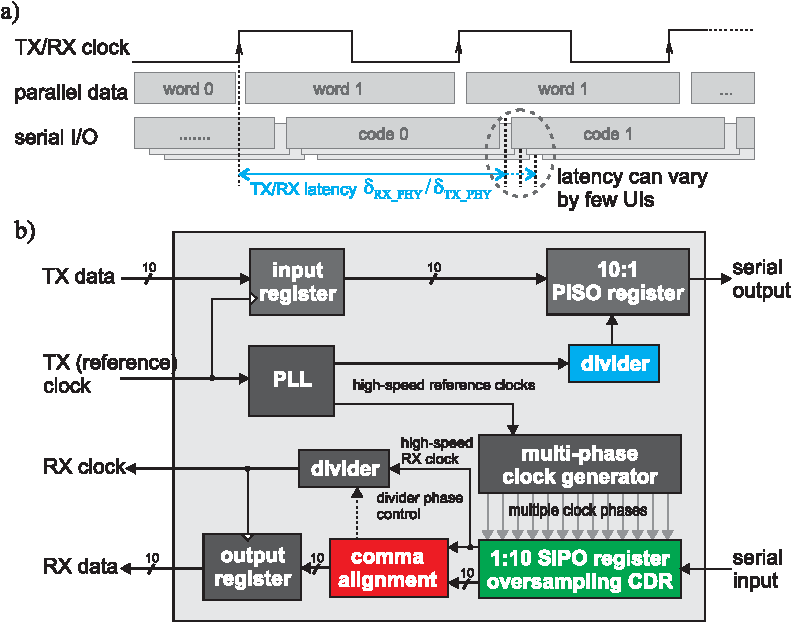
\includegraphics[width=11cm]{protocol/phy_asymmetry.pdf}
  \caption{Random delays in gigabit SerDes devices (a) and blocks causing them
  (b).}
  \label{fig:phy_asymmetry}
\end{figure}
PHY asymmetry manifests itself as a random latency between the rising edge of
the TX/RX clock and the inter-symbol boundary in the transmitted (received)
serial data stream. In most PHYs, this latency can be different for each
PLL/CDR lock cycle, but once the PHY is locked, the delays shall remain
constant. PHYs whose TX/RX delays can change when the link is active are
unsuitable for WR devices.

In the PHYs which have been evaluated for usability in WR hardware (TLK1221
from Texas Instruments and Virtex-6/Spartan-6 GTP transceivers), the following
random delays were identified:
\begin{itemize}
\item RX alignment latency, observed in PHYs which do not correct the RX
clock phase when aligning to the inter-symbol boundary (red, observed for
Xilinx GTP),
\item RX latency resulting from the internal structure of the digital
oversampling CDR (green, observed for TLK1221),
\item TX latency caused by the clock divider between the internal PLL and
the parallel-to-serial register (blue, observed for TLK1221).
\end{itemize}
Alignment latency can be measured every time the link goes up by disabling
automatic comma alignment and bit-shifting the unaligned output data
until a valid 8B10B code sequence is detected (\textit{bitslip trick},
see \cite{Peek2010}). Compensation of the latter two latencies, however,
requires additional calibration logic. An example method (used in the WR
switch) is shown in Figure~\ref{fig:phy_latency_measurement}.
\begin{figure}[ht!]
  \centering
%  \includegraphics[width=\textwidth]{fig/tomeksDrawings/phy_latency_measurement.eps}
	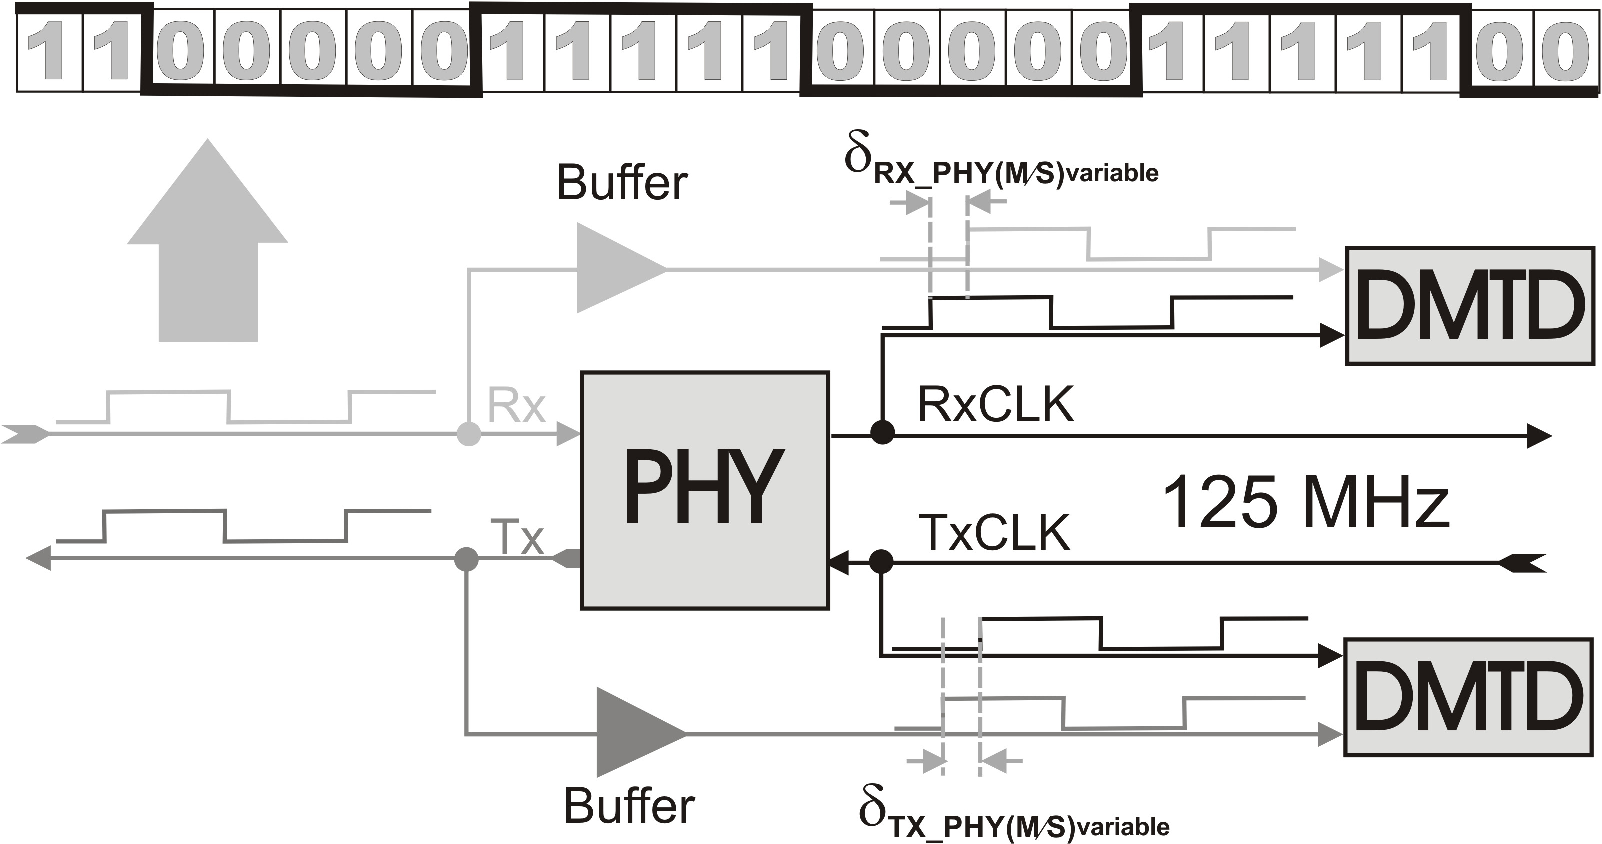
\includegraphics[width=0.60\textwidth]{misc/calibration_1.pdf}
  \caption{PHY latency measurement using calibration patterns.}
  \label{fig:phy_latency_measurement}
\end{figure}
Such methods can by applied to the
PHYs whose maximum ($\delta_{PHY(M/S)_{max}}$) and minimum ($\delta_{PHY(M/S)_{min}}$) delays are known 
(provided in the datasheet) and the delay's variation is
\begin{equation}
  \label{eq:fixedDelayVariation}
  \delta_{\{TX, RX\}\_PHY(M/S)_{variable}} \in \langle 0 :\delta_{PHY(M/S)_{max}} - \delta_{PHY(M/S)_{min}} \rangle
\end{equation}
e.g. below 10 bit times in the case of Gigabit Ethernet. 
Therefore, a fixed delay can be expressed as a sum of a constant value 
($\delta_{\{TX, RX\}\_PHY(M/S)_{min}}$) and a variable part ($\delta_{\{TX, RX\}\_PHY(M/S)_{variable}}$) which needs to be measured:
\begin{equation}
  \label{eq:fixedDelay}
  \delta_{\{TX, RX\}\_PHY(M/S)} = \delta_{\{TX, RX\}\_PHY(M/S)_{min}} + \delta_{\{TX, RX\}\_PHY(M/S)_{variable}}
\end{equation}
 


The PHY transmit path is fed with a sequence of RD+ K28.5 characters (1111100000),
effectively producing a 125 MHz square wave on the serial outputs. 
The repeated pattern of five "0" and five "1" is defined by the IEEE 802.3 standard \cite{IEEE802.3} 
as \textit{Low-frequency test pattern} (Appendix~36A.2). The phase
shift between the TX clock and the output bitstream can be measured using
a DDMTD phase detector, giving the value of the TX variable latency 
($\delta_{TX\_PHY(M/S)_{variable}}$). The same method
can be used to measure the RX variable latency ($\delta_{RX\_PHY(M/S)_{variable}}$) 
by commanding the link partner to send
the calibration pattern. Note that since the K28.5 character contains a comma
(5 consecutive ones), a burst of subsequent K28.5 symbols will cause improper
operation of the PHY's comma alignment unit. Therefore, comma alignment must
be disabled during the calibration process.

\subsection{Establishing and maintaining synchronization}
\label{s:estab_sync}
Having obtained the values of round-trip delay $delay_{MM}$ and link asymmetry,
we can calculate the one-way master to slave delay $delay_{MS}$ by solving
equation (\ref{eq:delaymm_full}):

\begin{equation}
delay_{MM} = \Delta + \delta_{ms} + \delta_{sm}
\label{eq:delaymm_full}
\end{equation}

where $\Delta = \Delta_{txm} + \Delta_{rxs} + \Delta_{txs} +
\Delta_{rxm}$. Substituting $\delta_{sm}$ with \ref{eq:fiber_alpha1}
and solving for $\delta_{ms}$, we obtain the one-way fiber delay
\ref{eq:delaymm_full_2}:

\begin{equation}
\delta_{ms} = \frac{1+\alpha}{2+\alpha} (delay_{MM} - \Delta)
\label{eq:delaymm_full_2}
\end{equation}

which after adding the circuit, SFP and PHY asymmetric delays present on the
master to slave path gives the final master-slave delay \ref{eq:delaymm_full_3}
and offset \ref{eq:offset_ms}:

\begin{eqnarray}
\label{eq:delaymm_full_3}delay_{MS} & = & \frac{1+\alpha}{2+\alpha} (delay_{MM}
- \Delta) + \Delta_{txm} + \Delta_{rxs} \\
\label{eq:offset_ms} offset_{MS} & = & t_{1} - t_{2p} - delay_{MS}
\end{eqnarray}
The value of $offset_{MS}$ is the input for the slave's offset adjustment
algorithm which controls the slave's clock servo. The flow diagram of the
algorithm is shown in fig. \ref{fig:adjustment_and_servo}a and an example
servo design can be found in fig. \ref{fig:adjustment_and_servo}b. The
algorithm assumes that the frequency has been already syntonized by means
of Sync-E and only the clock offset needs to be corrected. Offset correction
is split into 3 steps:
\begin{figure}[ht!]
  \centering
  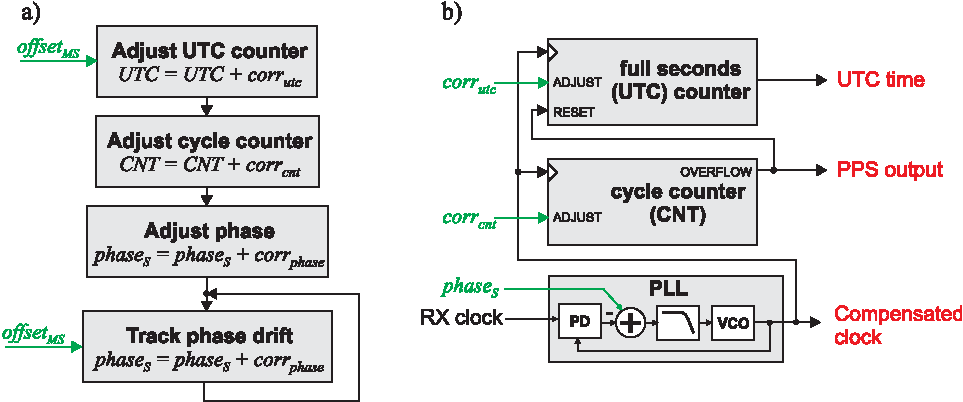
\includegraphics[width=\textwidth]{protocol/adjustment_and_servo.pdf}
  \caption{WR slave offset adjustment (a) and clock servo (b)}
  \label{fig:adjustment_and_servo}
\end{figure}
\begin{enumerate}
\item \textbf{UTC time adjustment}: the UTC counter in the servo is
increased (or decreased) by the number of full seconds \ref{eq:corr_utc}
in $offset_{MS}$:
\begin{equation}
corr_{utc} = \lfloor{\frac{offset_{MS}}{1 \mathrm{~s}}}\rfloor
\label{eq:corr_utc}
\end{equation}
\item \textbf{Clock cycle counter adjustment}: The reference clock cycle
counter, which produces the PPS signal is adjusted by the number of full
$T_{ref}$ (8 ns) cycles \ref{eq:corr_cnt}.
\begin{equation}
corr_{cnt} = \lfloor \frac{offset_{MS} - corr_{UTC}}{T_{ref}}\rfloor
\label{eq:corr_cnt}
\end{equation}
\item \textbf{Phase adjustment}: The slave's phase shifter is adjusted with
the remaining sub-cycle part of the offset \ref{eq:corr_phase}
\begin{equation}
corr_{phase} = offset_{MS} - [offset_{MS}]
\label{eq:corr_phase}
\end{equation}
\end{enumerate}
\emph{Voil\`{a}!} Now the slave's clock and PPS signals are synchronized to the
master with sub-nanosecond accuracy. Since the offset can vary with operating
conditions, it is measured at regular intervals and the difference between
subsequent measurements is added to the slave's phase shift to compensate for
phase drift:
\begin{equation}
corr_{phase} = offset_{MS} - offset_{MS\us previous}
\label{eq:corr_phase2}
\end{equation}
Because the phase drift is mainly caused by temperature variations, the rate
of subsequent adjustments can be very low, even in the scale of a single
adjustment per hour.

Note that the way $corr_{phase}$ is calculated requires the phase shifter
to be able to change the phase relatively by any arbitrary value with
no "jumps" in the signal when the value of $corr_{phase}$ crosses the
inter-cycle boundary. For example, one can use a PLL with a phase detector
capable of handling wrap-around phase transitions, but not a programmable
delay line. An example design of such phase detector and PLL is described
in section 4.3.7 of \cite{tomekMSC}.

